\documentclass{article}
    % General document formatting
    \usepackage[margin=0.7in]{geometry}
\usepackage[parfill]{parskip}
\usepackage[utf8]{inputenc}

% Related to math
\usepackage{amsmath,amssymb,amsfonts,amsthm}
\usepackage{graphicx}
\usepackage{enumitem}
\usepackage{tikz}
\usepackage{xcolor}
\usepackage{gensymb}
\setenumerate[1]{label=\thesubsection.\arabic*.}
\setenumerate[2]{label*=\arabic*.}


    % TODO: change thesis information
    \newcommand*{\getOrganisation}{Student Airrace}
    \newcommand*{\getTitle}{Technical Regulations}
    \newcommand*{\getAuthor}{Orga team}
    \newcommand*{\getDate}{12.01.2023}
    \newcommand*{\getVersion}{v0.1}
    \newcommand*{\getLocation}{Munich}
  

\begin{document}


\begin{titlepage}
    % HACK for two-sided documents: ignore binding correction for cover page.
    % Adapted from Markus Kohm's KOMA-Script titlepage=firstiscover handling.
    % See http://mirrors.ctan.org/macros/latex/contrib/koma-script/scrkernel-title.dtx,
    % \maketitle macro.
    \oddsidemargin=\evensidemargin\relax
    \textwidth=\dimexpr\paperwidth-2\evensidemargin-2in\relax
    \hsize=\textwidth\relax
  
    \centering
  
    \IfFileExists{logos/STAR_logo.png}{%
      
\includegraphics[height=20mm]{logos/STAR_logo.png}
    }{%
      \vspace*{20mm}
    }
  
    \vspace{5mm}
    {\huge\MakeUppercase{\getOrganisation{}}}\\
  
    \vspace{5mm}
  
    \vspace{20mm}
  
    \vspace{15mm}
    {\huge\bfseries \getTitle{}}
  
    \vspace{15mm}
    {\getDate{}}
    \vspace{10mm}
    \linebreak
    {\getVersion{}}
    \linebreak
    { \getLocation{}}
  
  
  
  
  
    \IfFileExists{logos/tum_logo.png}{%
    \vfill{}
    
\includegraphics[height=20mm]{logos/tum_logo.png}
      }{}
  \end{titlepage}

\tableofcontents{}

\newpage
{\bf Authors}
\\ \\Janis Mauch \emph{\\Founder of Student AirRace - Regulations Team \\janis.mauch@student-airrace.com}
\\ \\ Simon Pokorny \emph{\\Cofounder of Student AirRace - Technology Team \\simon.pokorny@student-airrace.com}
\\ \\ \\
{\bf Changelog}
\\ \\{\bf Current Version: \\Version Draft \getVersion{}}
\\ \\Previous Versions: \\ No previous Versions

\newpage
{\bf Preface}
\\ \\ Welcome to the Student AirRace competition! \\ \\
Get ready for an adrenaline-pumping experience as you showcase your talents and skills in the thrilling world of drone racing. 
For our team, this competition has been a dream come true, and we are honored to host it. 
At Student AirRace, our vision is to become the premier air race competition for students and one day, maybe even evolve into manned aircraft competitions.
\\ \\ 
Safety is our top priority, and we are dedicated to ensuring that all participants and spectators have a safe and unforgettable experience. 
We understand that the technology and regulations surrounding drones, eVTOLs, and UAS are constantly evolving, and we have done our best to create regulations that are comprehensive and up-to-date with the current state of the industry. 
However, we also understand that there is always room for improvement, and we welcome any feedback you may have to help us make this competition even better.
\\ \\ 
We have put a lot of hard work and dedication to get to this point and we can't wait to see what you have to bring to the table. 
We hope you will not only have fun, but also learn a lot and make valuable connections in the industry. 
Get ready to push your limits and soar to new heights as we witness the innovative solutions and ideas you will bring to the competition. 
Welcome to the racing of the future. You are now a part of it.
\\ \\ \\
Janis Mauch 
\\ \\Founder of Student AirRace


\newpage
{\bf Notes:
\begin{itemize}
  \item Contents marked in \textcolor{red}{red} are still subject to change and should be seen as current estimations and placeholders.
  \item This whole document is still a work in progress. Some points may still be left empty.
  \item If you have any comments on specific regulations, for example, think that they are not required, are too strict or don't make sense, don't hesitate to contact regulations@student-airrace.com.
\end{itemize}
}
\hspace{10mm}

{\bf Abbrevations:}
\begin{tabbing}
  {\bf AI~~~~~~~~~~~~~~} \= Artificial Inteligence
  \\{\bf ARP} \> Aeronautical Recommended Practices
  \\{\bf CE} \> Conformité Européene (European Conformity)
  \\{\bf DC} \> Direct Current
  \\{\bf EASA} \> European Union Aviation Safety Agency
  \\{\bf e-ID} \> electronic identification
  \\{\bf EU} \> European Union
  \\{\bf EU-LBT} \> EU Listen Before Talk
  \\{\bf EIRP} \> Equivalent Isotropically Radiated Power
  \\{\bf ESC} \> Electronic Speed Controller
  \\{\bf EUROCAE} \> European Organisation for Civil Aviation Equipment
  \\{\bf FPV} \> First Person View
  \\{\bf HITL} \> Hardware-in-the-loop
  \\{\bf ICAO} \> International Civil Aviation Organization
  \\{\bf ISO} \> International Organization for Standardization
  \\{\bf Lipo} \> Lithium Polymer
  \\{\bf LTE} \> Long-term Evolution
  \\{\bf MTOW} \> Maximum Take-Off Weight
  \\{\bf NOTAMS} \> Notice to Airmissions
  \\{\bf RC} \> Remote Control
  \\{\bf RTH} \> Return to Home
  \\{\bf SORA} \> Standard Operating Risk Assessment
  \\{\bf UAS} \> Unmanned Aerial System
  \\{\bf UAV} \> Unmanned Aerial Vehicle
\end{tabbing}




\newpage
\section{Definitions}
\subsection{Propeller Disks}
\begin{enumerate}
  \item The propeller disk is a cylinder within the Body-Fixed-Frame defined by the full rotation of a single propeller. Each propeller has its respective propeller disk. 
  \item The centre axis of this cylinder is referred to as the propeller shaft. Its intersection with the disk's centre will be used as a reference point for any measurements taken from the propeller disk. Every measurement which mentions the propeller disk within these regulations refers to this point.
\end{enumerate}

\begin{figure}[h!]
  \centering
   \IfFileExists{figures/RotorDiskExample.png}{%
   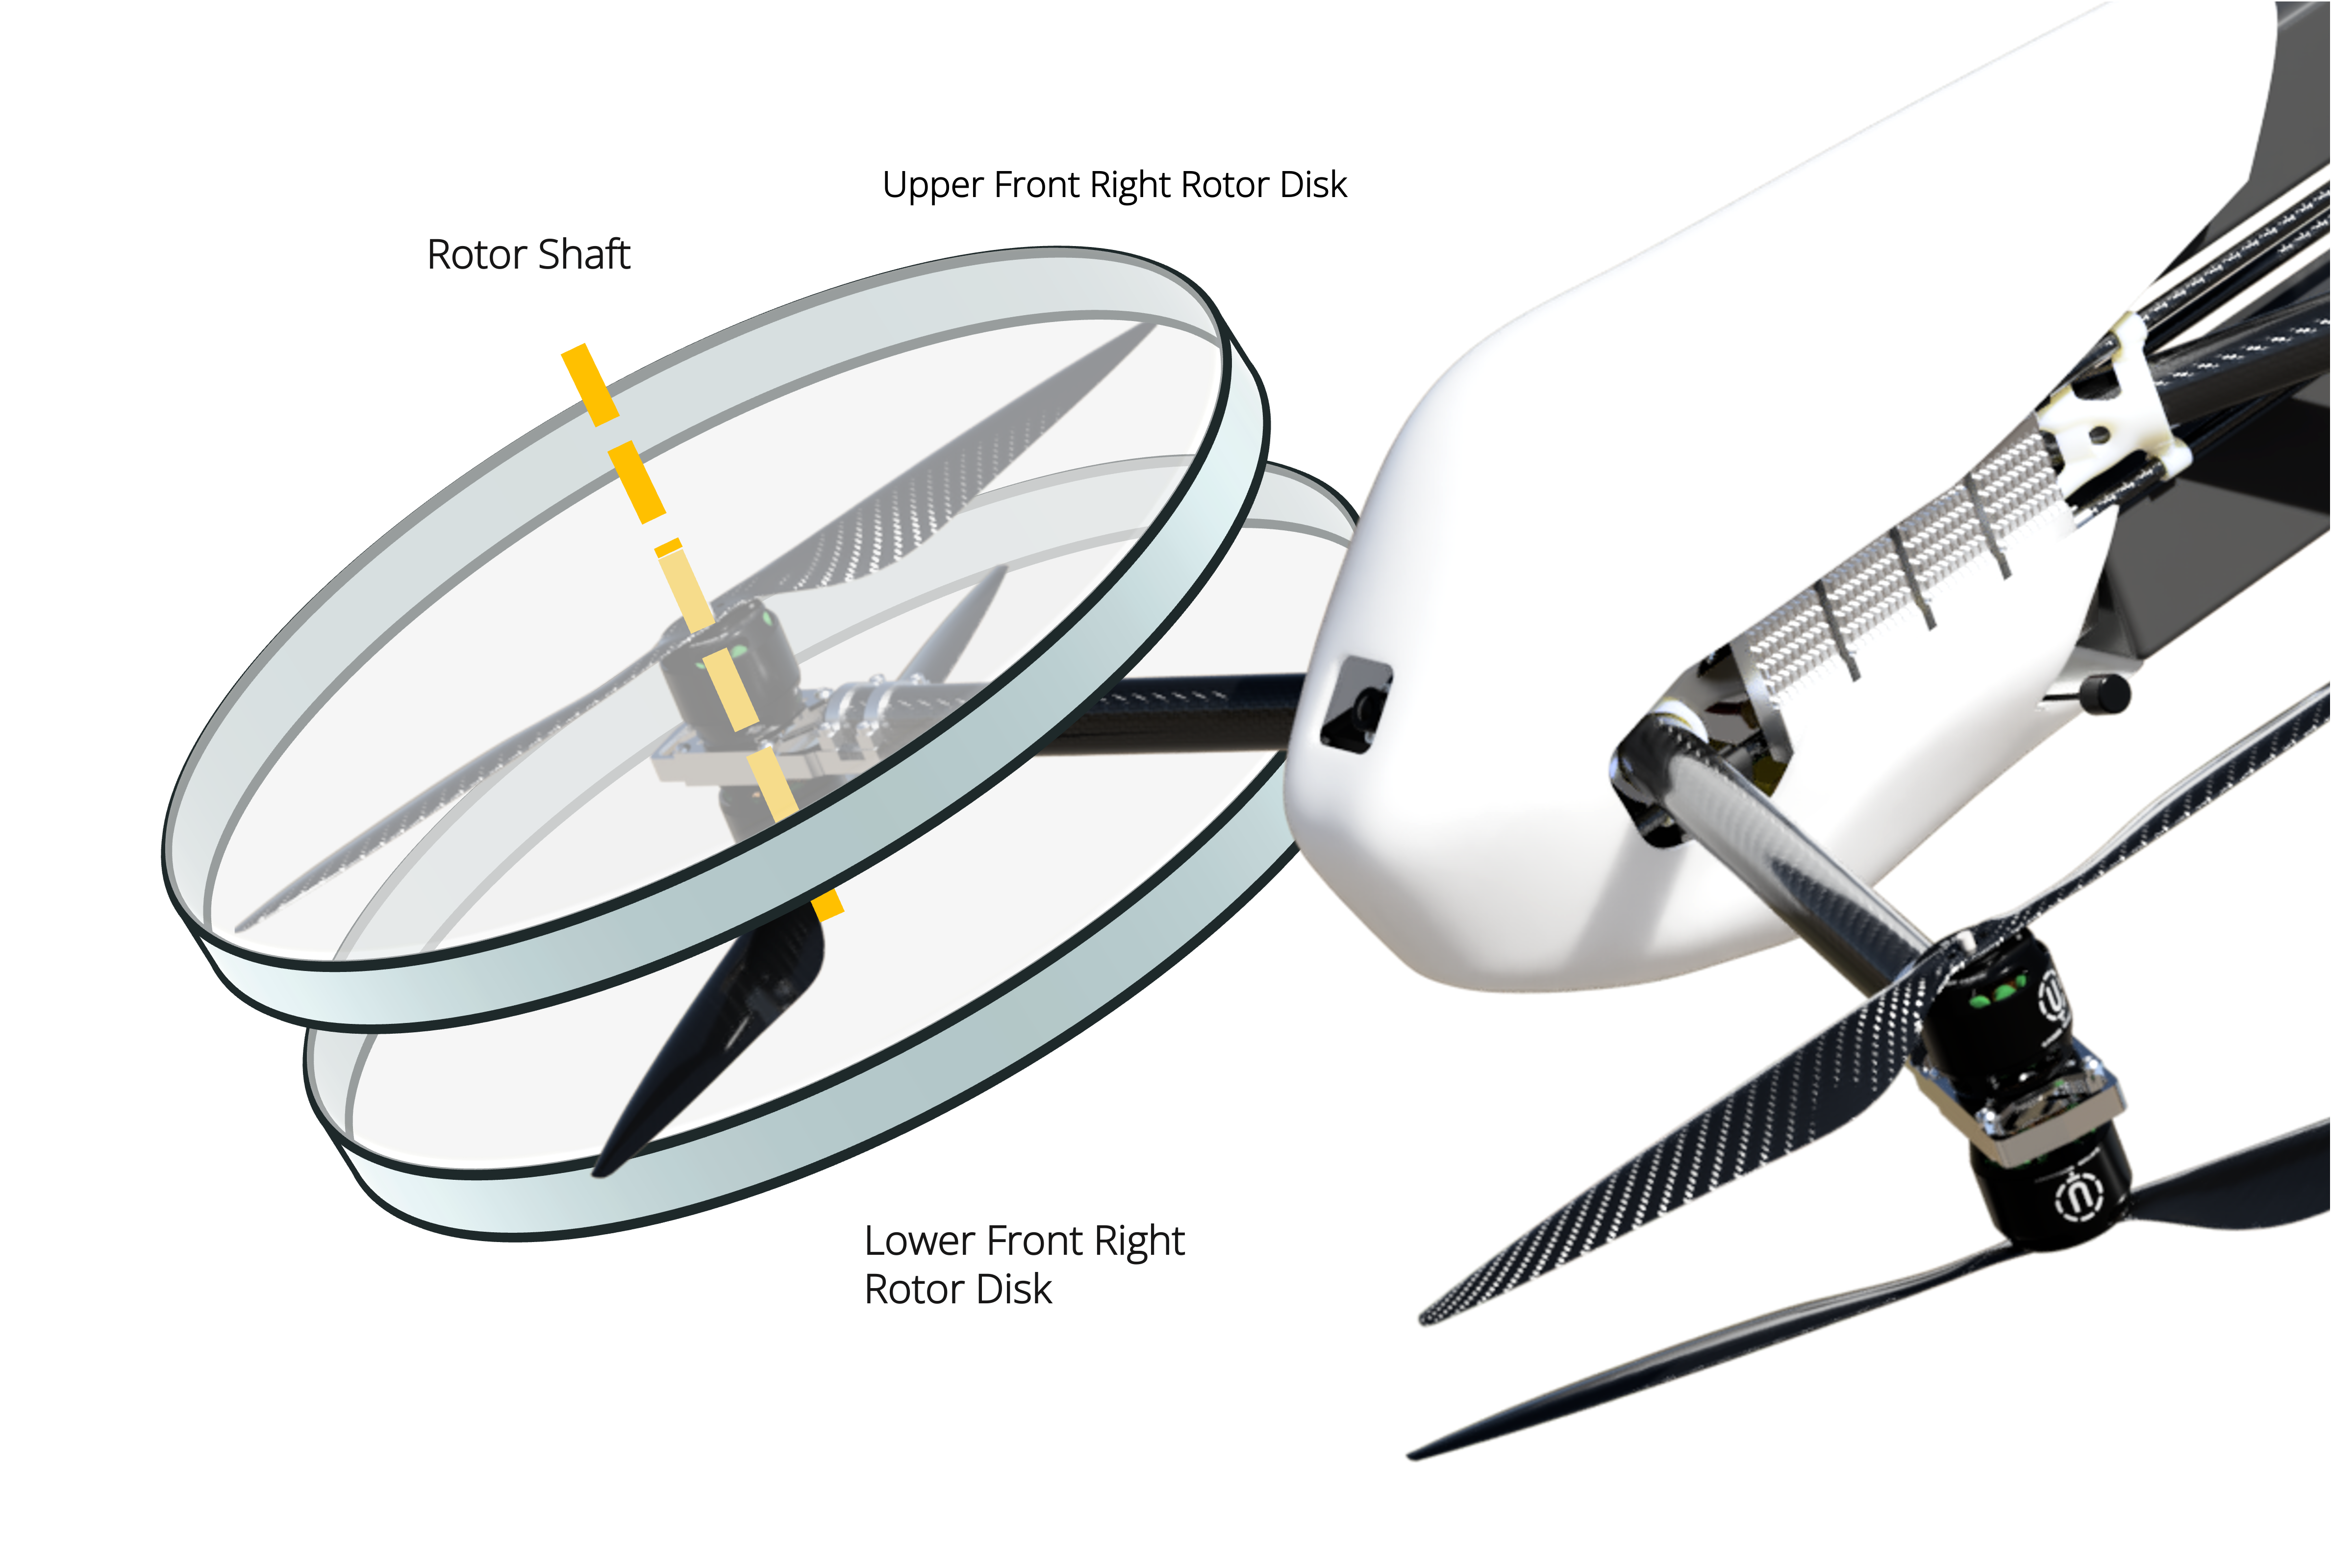
\includegraphics[height=70mm]{figures/RotorDiskExample.png}
   }{%
   \vspace*{70mm}
   }
 \caption{\textit{Example of the rotor disk on a generic drone.}}
 \end{figure}




\subsection{Vehicle Coordinate Frame Definitions}
\begin{enumerate}
  \item The Ground Plane is defined as the ground when the aircraft is in landed position with the landing gear extended. Even during flight, this plane stays fixed to the Body-Fixed-Frame of the aircraft.
  \item The XY-Plane is parallel to the ground plane. The intersection with the lowest propeller disk centre defines its exact position.
  \item Our axis are defined in a classical Aircraft Fixed Body System. The x-Axis is defined as being within the XY-Plane. It points (except for the azimuth angle) towards the intended direction of flight.
  \item The z-Axis is defined as an axis perpendicular to the XY-Plane. It intersects the XY-Plane in the aircraft's centre of gravity. As usual in a Body-Fixed Aircraft frame, the positive direction points downwards during the landed state.
  \item The y-axis is defined with the right-hand rule as an orthonormal vector on the X and Z vectors.
  \item The Coordinate frames must be marked and made visible in the competitor's technical report. 
  
  \begin{figure}[h!]
    \centering
     \IfFileExists{figures/CoordinateFrame.png}{%
     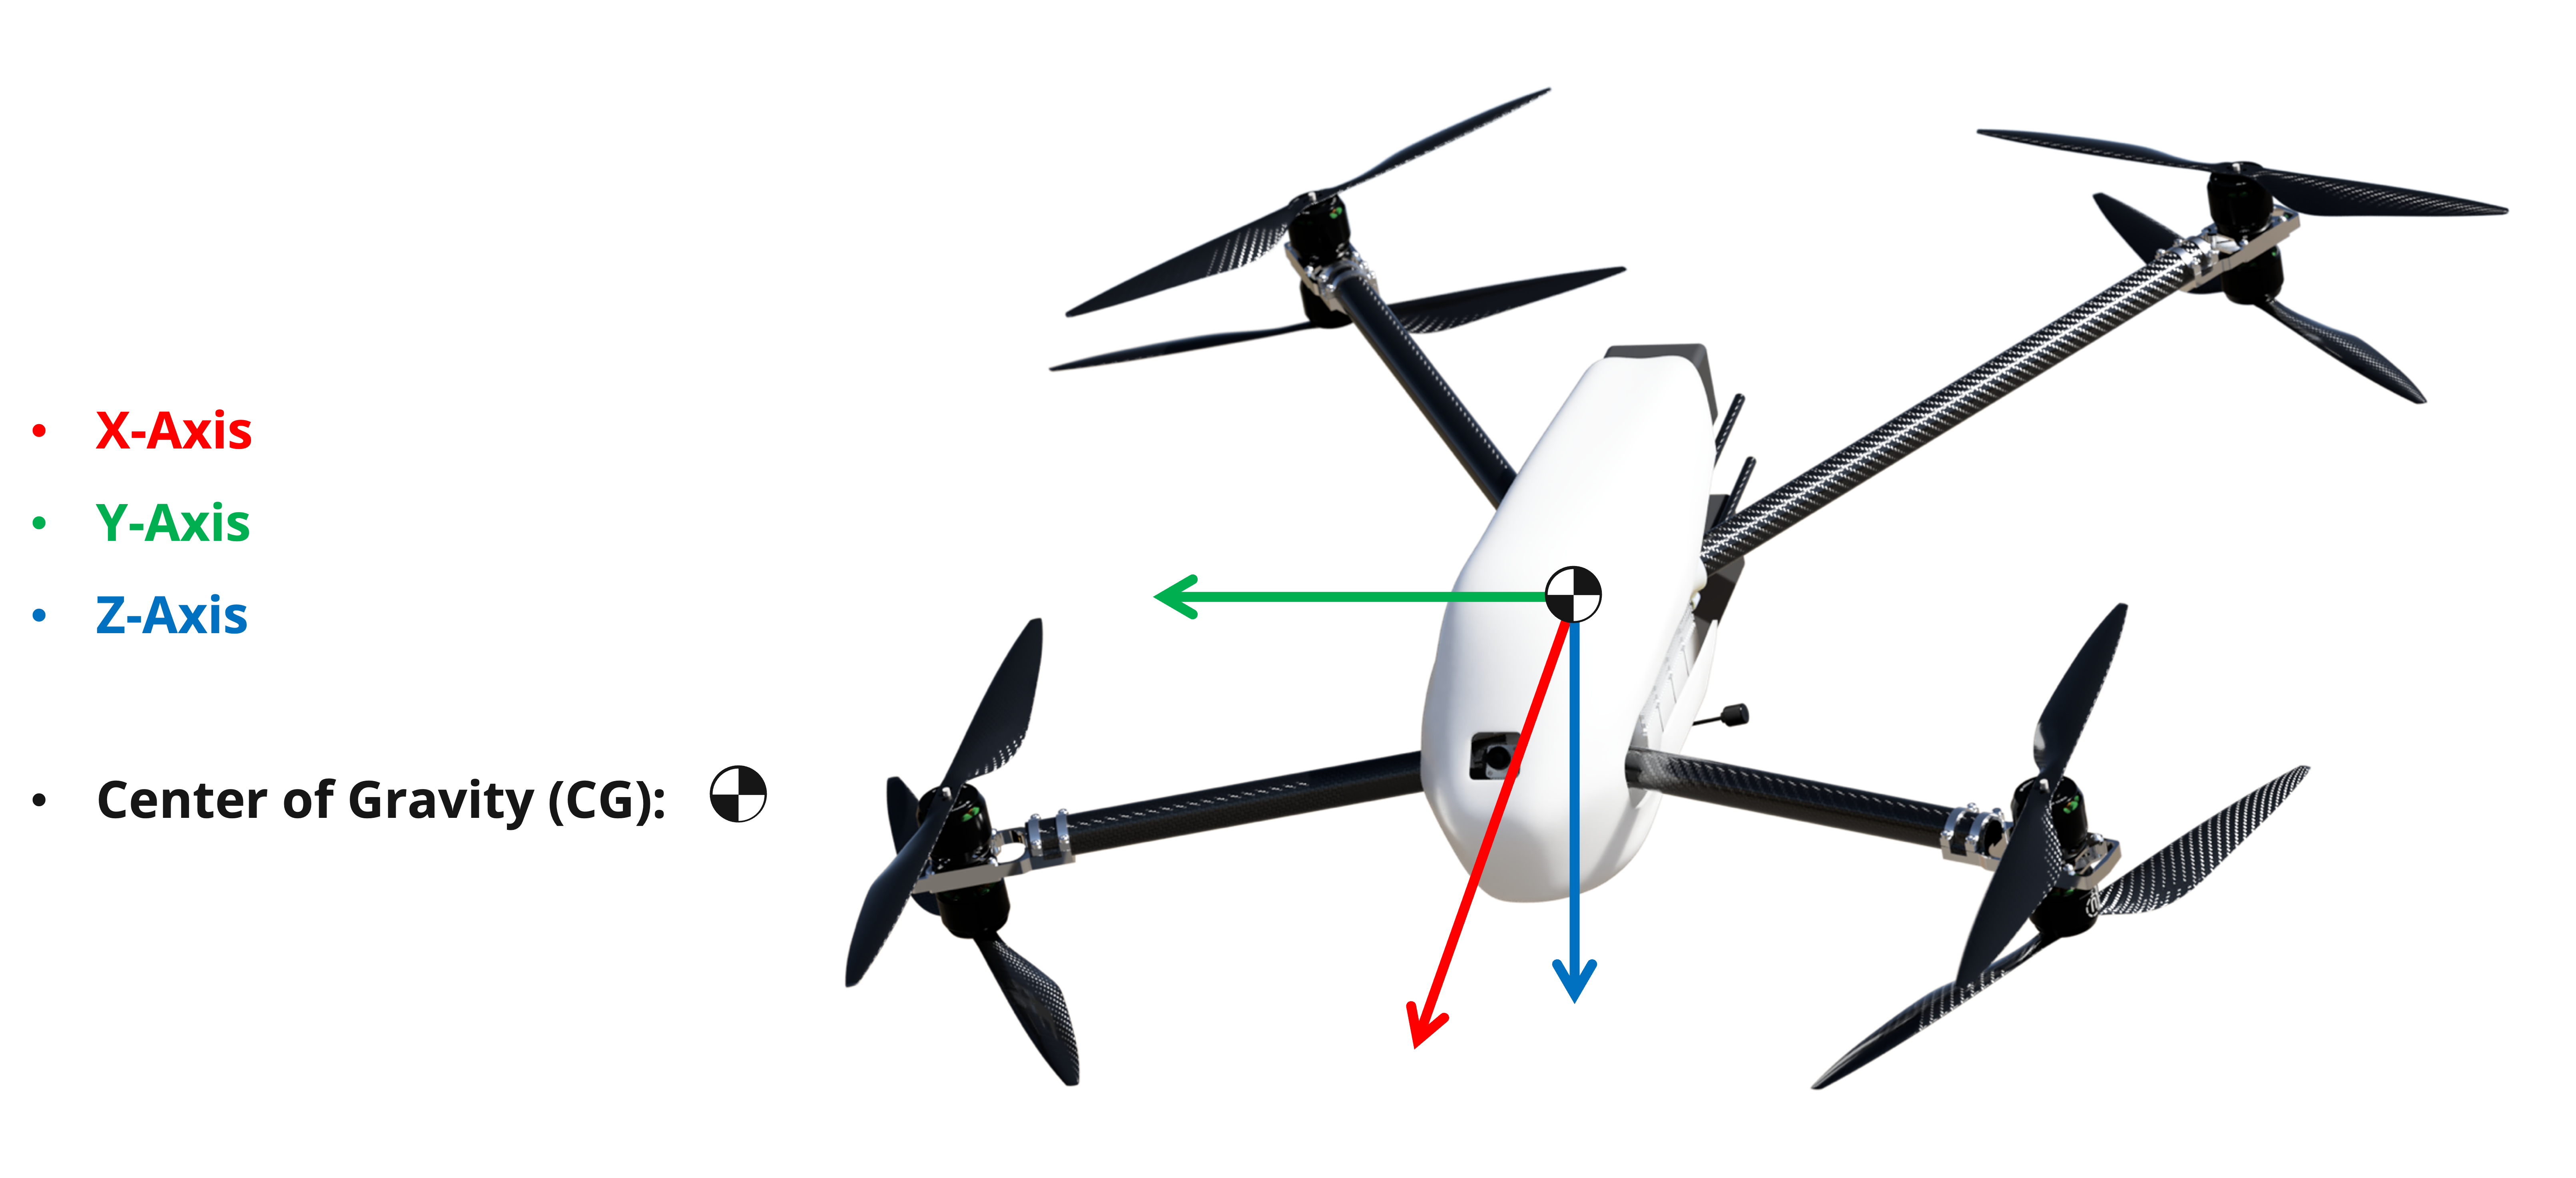
\includegraphics[height=50mm]{figures/CoordinateFrame.png}
     }{%
     \vspace*{50mm}
     }
   \caption{\textit{Coordinate Frame Example on a generic drone.}}
   \end{figure}
\end{enumerate}

\subsection{Power Units}
\begin{enumerate}
  \item A power unit is a lift-producing actuator associated with control electronics. A classical multicopter design would include a single electronic speed controller (ESC) on the aircraft, the motor it controls, and the attached propeller. Each of these components constitutes a single powertrain. 
  \item To ensure that only legitimate power units are used in the competition, all devices declared power units must be strictly used to produce thrust. Any components used for cooling or other purposes will not be considered power units.
\end{enumerate}


\newpage
\newpage

\section{Environmental Envelope}
Teams can only fly their aircraft if they meet operational conditions and requirements. These conditions must be fully satisfied before any flights may be conducted:
\begin {itemize}
  \item The aircraft must be able to operate in temperatures between \textcolor{red}{5 \degree C} and \textcolor{red}{30 \degree C}.
  \item The relative humidity must stay within \textcolor{red}{0\%} and \textcolor{red}{100\%}. 
  \item The aircraft must be able to operate within a range of air pressures, with a minimum of \textcolor{red}{950 hPa} and a maximum of \textcolor{red}{1050 hPa}.
  \item The average windspeed must stay below \textcolor{red}{6m/s}. Gusts may not exceed \textcolor{red}{15m/s} within one hour before and during the flight.
  \item The aircraft must be designed and built to withstand flying in drizzle conditions, including maintaining stability and control and protecting sensitive equipment from moisture despite precipitation.
  
\end {itemize}


\section{Aircraft Performance Requirements}

\subsection{Vehicle Maximum Takeoff Weight (MTOW)}
\begin{enumerate}
  \item The Maximum Weight of the vehicle during scrutineering must not exceed 22.5kg.
  \item The Organizer will publish the weights of equipment which must be used during the competition and thus added to the vehicle beforehand. Those weights wound count towards the maximum weight. 
  However, the teams should plan their calculations for the vehicle with those weights added. The Maximum Takeoff Weight with this Equipment will not pass 25kg.  
  \item The Weight of the vehicle during scruteneering must exceed \textcolor{red}{12kg}.  
\end{enumerate}

\subsection{Vehicle Thrust}
\begin{enumerate}
  \item The minimum Thrust measured on the vehicle Thrust Test Stand must exceed \textcolor{red}{300N} under standard atmospheric conditions.
  \item If the atmospheric conditions during testing do not meet the ICAO standard atmosphere conditions, a correction factor based on the current air density will be applied to the thrust stand results linearly.
\end{enumerate}


\section{Electronics}


\subsection{Power Source}
\begin{enumerate}
  \item The aircraft's power source must be electric. All motors and actuators on the aircraft must also be electrically driven.
  \item Vehicles powerd by combustion engines, \textcolor{red}{Hydrogen Cells or comparable fuel burning devices} are not permitted. 
\end{enumerate}

\subsection{Onboard Electronics}
\begin{enumerate}
  \item The maximum Direct Current (DC) voltage across any two electrical connections on the aircraft must not exceed 60V.
  \item Team participants are permitted to use various battery types on their drones, provided that the batteries comply with EASA regulations for Unmanned Aerial Vehicles (UAV) and do not present a significantly elevated level of risk when compared to the use of a Lithium Polymer (Lipo) battery. 
  \item The total energy stored in a single battery may not exceed \textcolor{red}{40.000 mAh}.
  \item A fuse with a suitable current rating must be added in series with each battery in the propulsion system. 
  This fuse must be installed in line with the battery's positive terminal. Its maximum continuous current rating must be equal to or less than the maximum continuous discharge rating of the battery \textcolor{red}{times a safety factor of 1.3}. The goal is to protect the battery, the propulsion system, and the aircraft from damage or failure due to overcurrent conditions.
  \item At least two power sources must feed the flight control system. 
\end{enumerate}



\section{Aircraft Geometry}

\subsection{Vehicle Type}
\begin{enumerate}
  \item The vehicle must be able to take off and land vertically without posing a safety hazard or showing drift.  
\end{enumerate}

\subsection{Powerunit Posititons}
\begin{enumerate}
  \item The aircraft must have a minimum of 6 and may not have more than 16 power units. 
  \item The rotor disks can be offset to each other however the teams prefer within the XY-plane. 
  \item The furthest distance between two main-motor-shafts in x direction divided by the furthest distance between two main-motor-shafts in y direction must lie between \textcolor{red}{0.5 and 2}. 
  
  \begin{figure}[h!]
    \centering
     \IfFileExists{figures/MotorLayoutsXY.png}{%
     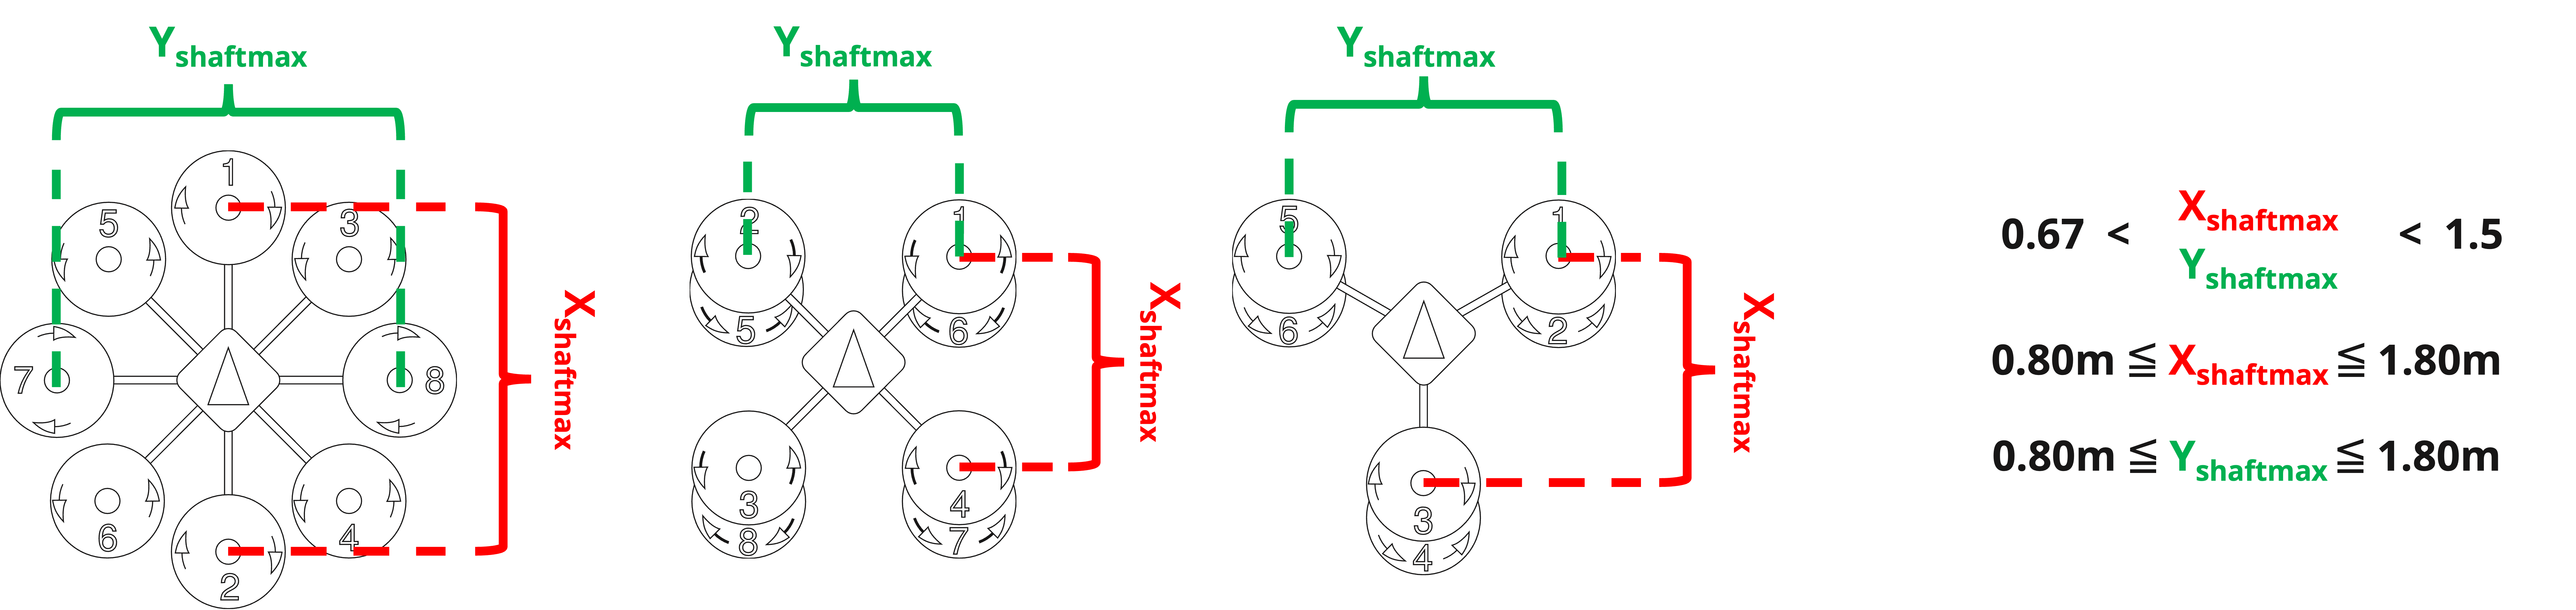
\includegraphics[height=35mm]{figures/MotorLayoutsXY.png}
     }{%
     \vspace*{35mm}
     }
   \caption{\textit{Examples of different rotor disk offsets within the XY-plane and their allowed distances.}}
   \end{figure}

  \item While the vehicle is standing on the ground with the landing gear extended, the lowest part of each propeller disk must have a ground clearance of at least \textcolor{red}{200mm}. 
  \item The rotor disks may be offset to each other in the z direction up until a maximum difference of +-400mm.
  
  \begin{figure}[h!]
    \centering
     \IfFileExists{figures/MotorLayoutZ.png}{%
     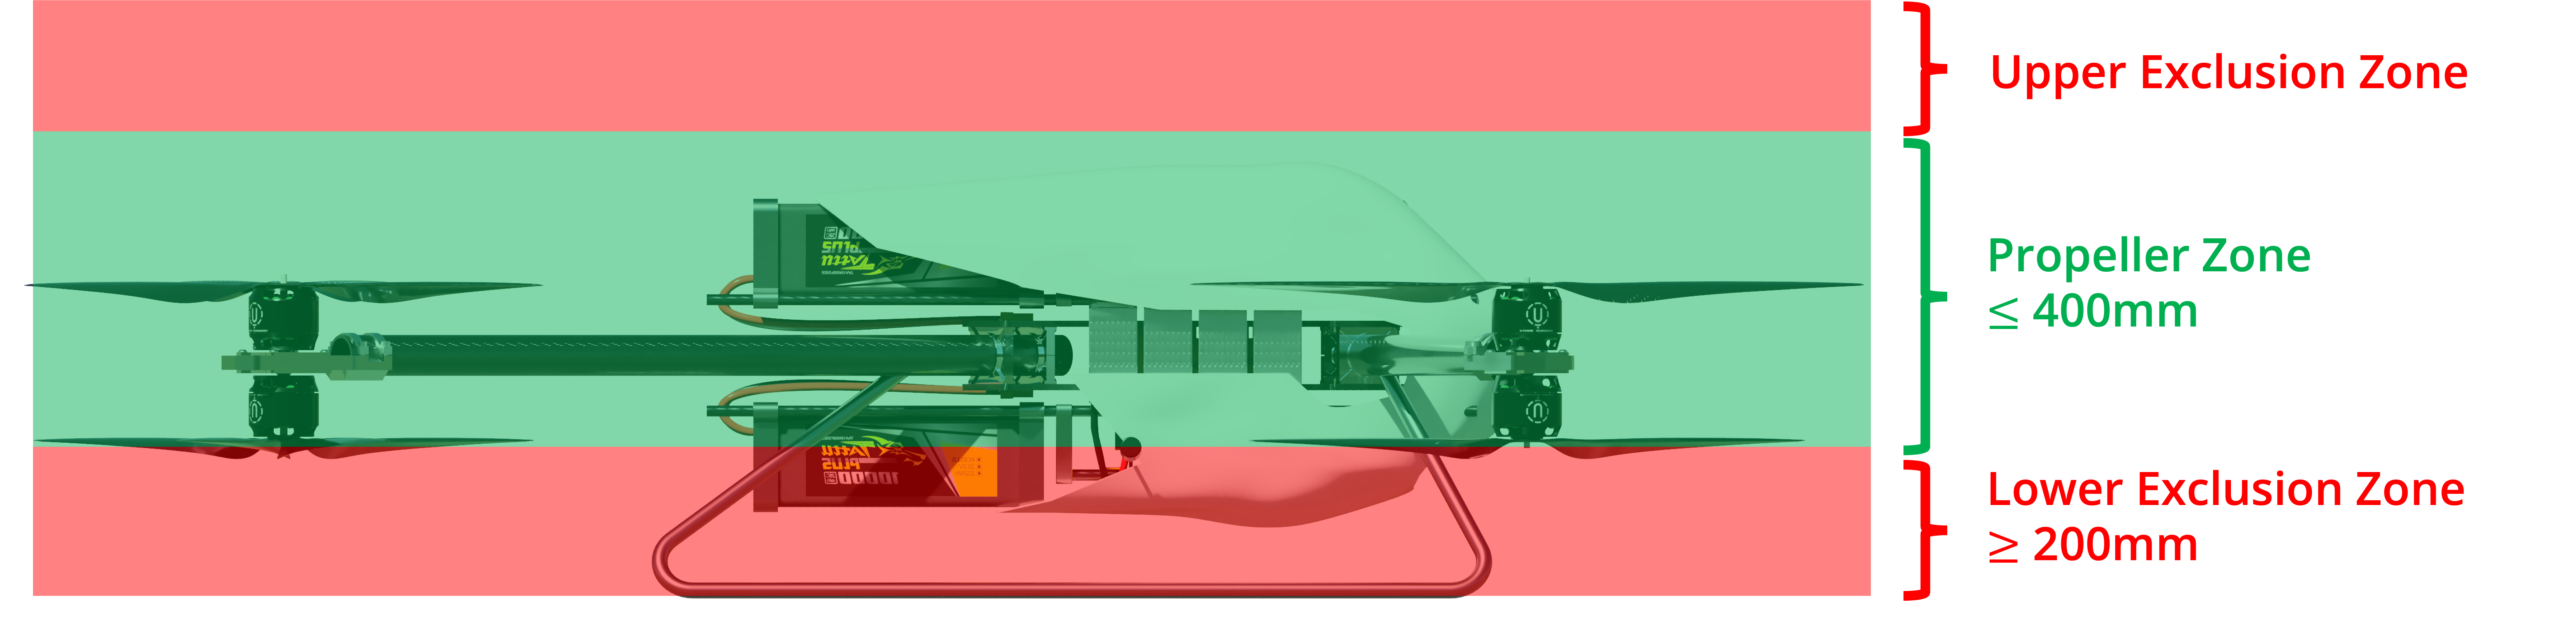
\includegraphics[height=35mm]{figures/MotorLayoutZ.png}
     }{%
     \vspace*{35mm}
     }
   \caption{\textit{Depiction of the power unit position in the z-axis and the resulting exclusion zones where no motors can be mounted.}}
   \end{figure}

  \item The rotor disks of the drone may overlap when viewed in the XY-Plane, as long as a necessary separation between the rotors during full thrust is ensured with a safety factor of 3 or more at the closest position. No additional proof is required if the distance between both disks exceeds at least 1/4 of the propeller diameter. However, if the distance between both disks is less than 1/4 of the propeller diameter, teams must provide proof in their safety report to demonstrate that the necessary separation is maintained.  \item Rotors in which rotor disks overlap or mesh within each other are not permitted. Even if mechanically or electronically coupled.
  \item The total vehicle size, including propeller disks, must not exceed a box with the side lengths of $x=3000mm$, $y=3000mm$, $y=1200mm$
  \item The full vehicle size, including propeller disks, must exceed a box with the side lengths of $x=1200mm$, $y=1200mm$, $y=300mm$

  \begin{figure}[h!]
    \centering
     \IfFileExists{figures/BoxSizesAircraft.png}{%
     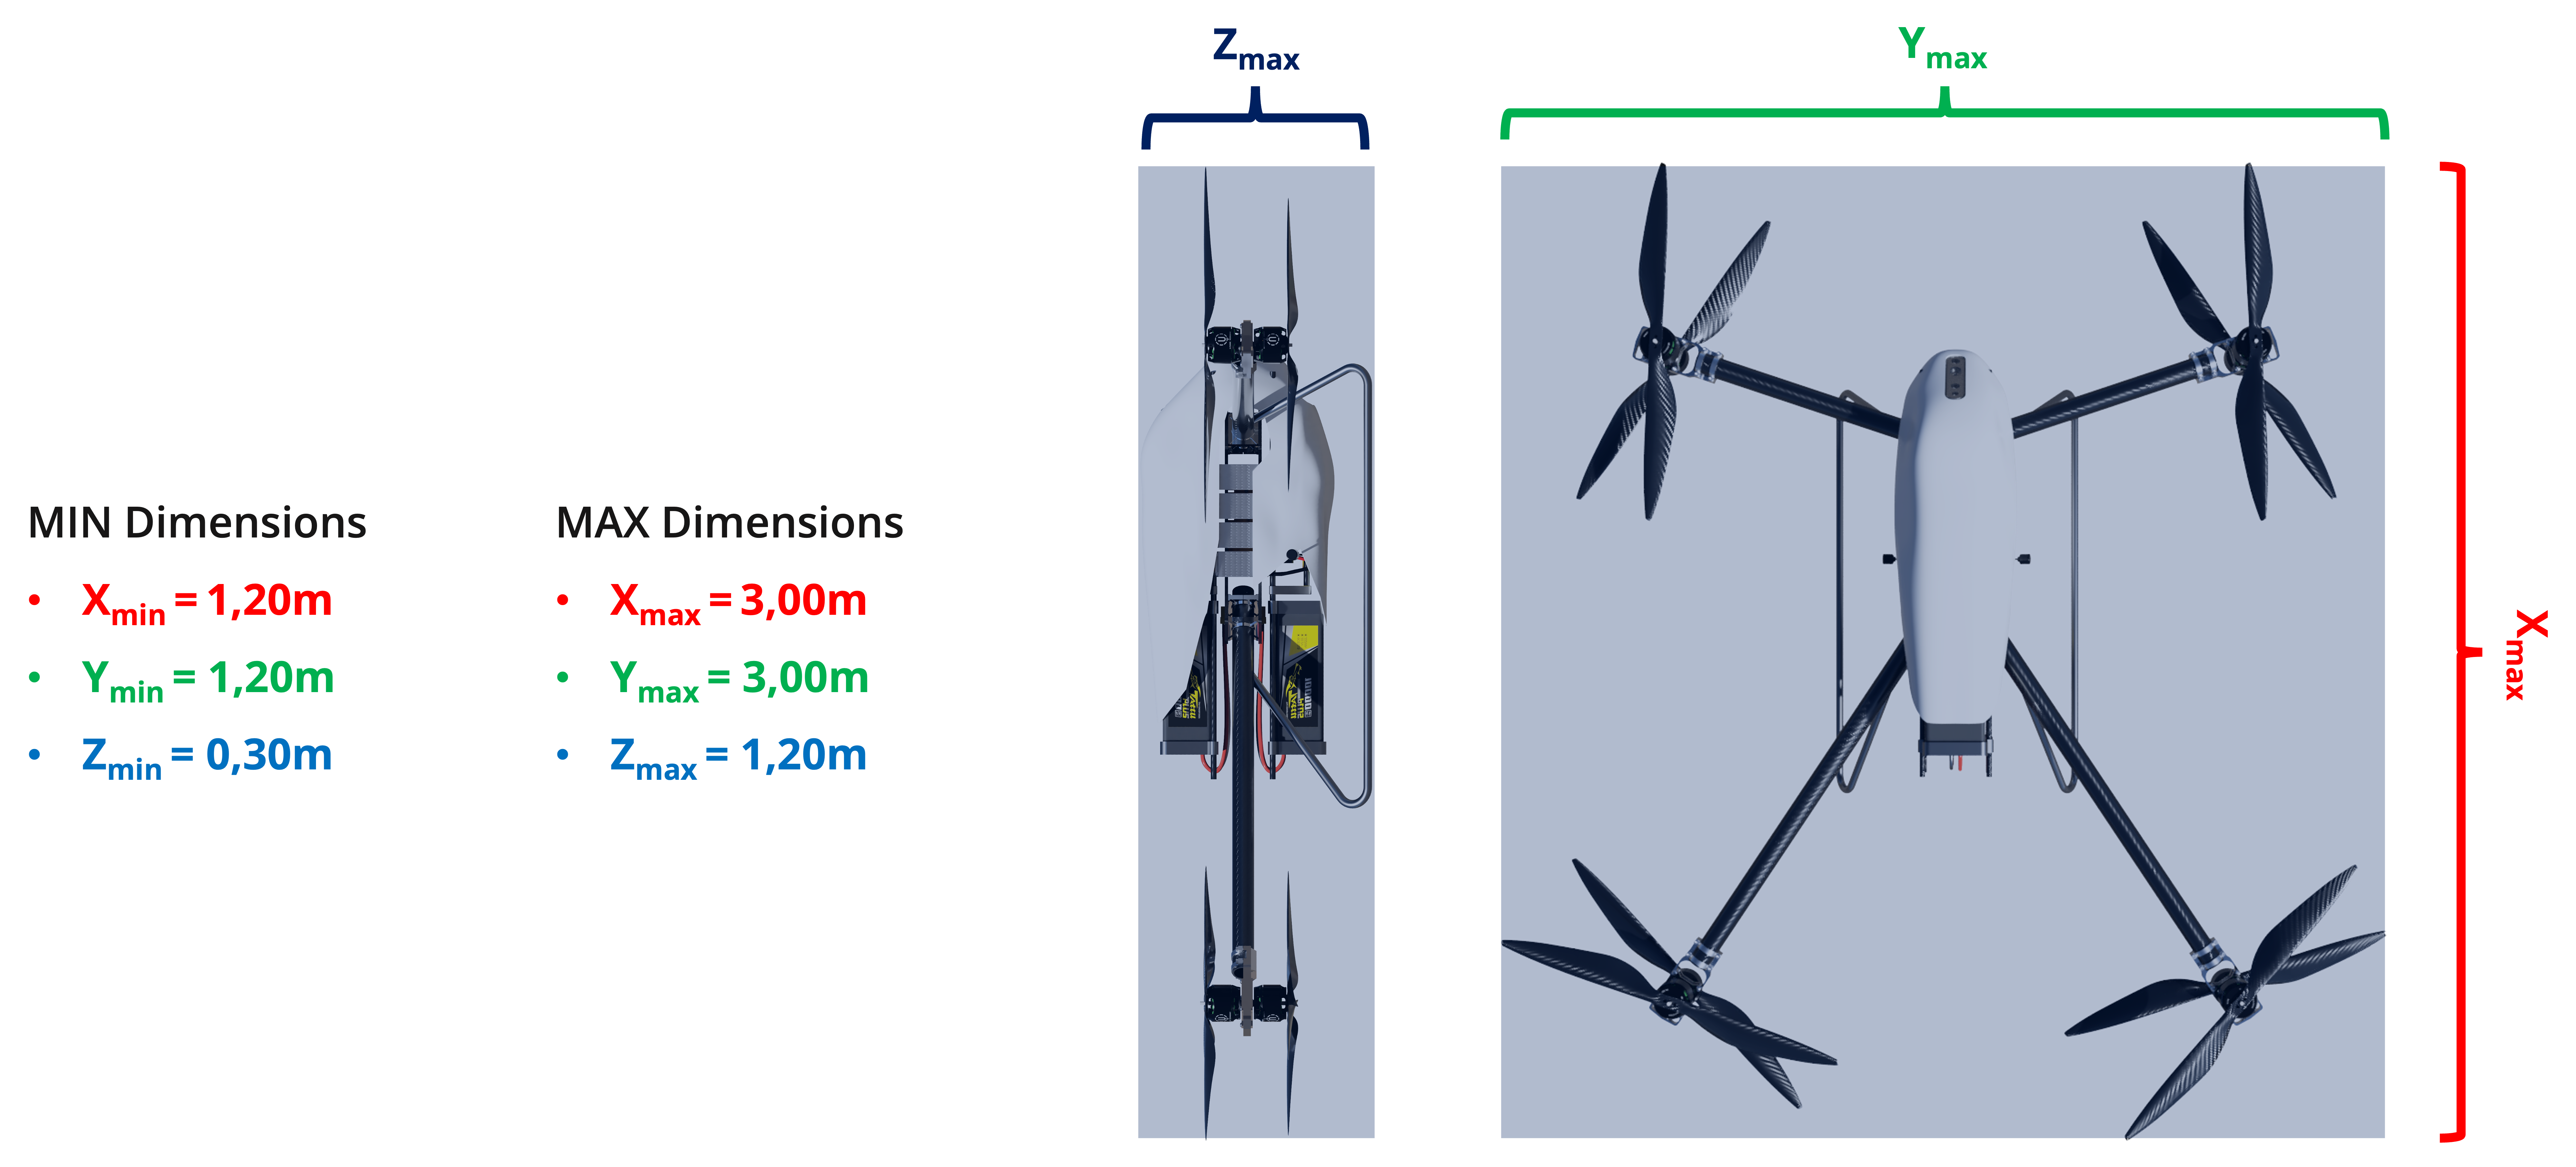
\includegraphics[height=60mm]{figures/BoxSizesAircraft.png}
     }{%
     \vspace*{60mm}
     }
    \caption{\textit{Minimum and Maximum sizes of the aircraft.}}
  \end{figure}
    
\end{enumerate}

\subsection{Powerunit/Motor Orientation}
\begin{enumerate}
  \item The motor shaft angle in relation to the vehicle's body frame must always be fixed during flight. 
  \item The motor shafts may be individually tilted by a maximum of \textcolor{red}{20\degree} parallel to the x-axis of the vehicle's body system. They must remain fixed, though.
  \item The motor shafts may be individually tilted by a maximum of \textcolor{red}{20\degree}  parallel to the y-axis of the vehicle's body system. They must remain fixed, though.
  \item The teams may use spacers to adjust these values to achieve different flight dynamics quickly.
\end{enumerate}


\subsection{Propeller Dimension}
\begin{enumerate}
  \item The minimum propeller diameter used on the main motors must exceed \textcolor{red}{$500mm$}.
  \item The maximum propeller diameter used on the main motors must not exceed \textcolor{red}{$1200mm$}.
  \item If varying propeller diameters are used on the main motors, the quotient must be within 0.67-1.5.
\end{enumerate}





\section{Aircraft Subsystems}

\subsection{Internal Cooling}
\begin{enumerate}
  \item Fans dedicated to cooling with a maximum diameter of 50mm can be fitted anywhere on the vehicle. These do not count as power units and thus do not need to follow the orientation rule from earlier.
  \item Water cooling is permitted. 
\end{enumerate}

\subsection{AI onboard computer}
These rules only apply if the competitor participates in the autonomy discipline.
\begin{enumerate}
  \item Every computation directly influencing the aircraft's trajectory must be executed onboard.
  \item The companion computer must be equipped with enough storage so that decisions made by the autonomy stack can be analysed afterwards in case of failure. 
  \item The navigation and trajectory planning algorithms must be validated in a Hardware in the loop(HITL) simulation before the race starts to ensure that the code works and the computer can process the workloads.
  \item A malfunction in the autonomy stack must result in a position-hold state. 
  \item Every sensor that perceives the environment must be onboard.
\end{enumerate}

\section{Liveries}
\begin{enumerate}
  \item The teams are responsible for ensuring that the university's logo, which operates the UAV, is visible from the front, left, and right sides of the aircraft. The logo must be at least fifty (50) mm in its smallest dimension  \item The competitors' number must be readable from any the front. It shall not be smaller than one hundred fifty (150) mm in its smallest dimension.
  \item The teams are allowed to display sponsor logos and another branding on their UAS if they do not contain any inappropriate or political messages or images. If the teams wish to include such content, they must coordinate with the organisers to ensure it is acceptable. 
  \item The teams are free to design the livery in their own style and team colours as long as the other rules are adhered to. 
\end{enumerate}


\section{Groundstation}
\subsection{Video Transmission}
\begin{enumerate}
  \item The teams must use a digital video connection suitable for flying an aircraft at the competition. 
  \item A spotter must always stand next to the pilot, especially when flying in First Person View (FPV). The spotter's role is to assist the pilot by maintaining a visual on the UAV's flight path, monitoring the airspace and providing an additional set of eyes to detect any potential hazards
  \item The video transmission method must be legal to use in Germany, which includes following the officially allowed frequencies and power outputs and having a valid CE certificate for the video system.
  \item \textcolor{red}{A secondary redundant video link must be in place. This rule might change. Tests will have to show whether two video links can work without affecting each other.}
\end{enumerate}

\subsection{External Cooling and Heating}
\begin{enumerate}
  \item Teams may use leafblowers or comparable devices to cool their aircraft after a flight externally. However, the aircraft must not be powered anymore and shut down, and the shunt plug must be disconnected.  
  \item Teams may preheat their batteries to an optimum operating temperature with external tools such as heating boxes or heating blankets.
\end{enumerate}

\section{Standardized Parts}

\subsection{T-Camera-Pod}
\begin{enumerate}
  \item The teams will have a standardised camera and sensor housing on top of the UAS.
  \item \textcolor{red}{The exact dimensions and the interface will still be designed and published. For now, four 4.5mm through holes through which M4 screws can be put and countered on the back with nuts can be assumed. They should be on a flat area and oriented on a circle with 60mm.}
  \item The combined mounting time of the T-Camera-Pod and external black box must not exceed 30 minutes at the competition. 
\end{enumerate}



\subsection{External Blackbox}
The external black box is a box that can be considered a sort of payload for the vehicle. The teams must leave space to fit it into their design.
\begin{enumerate}
  \item It will have two XT90 inputs and two XT90 outputs. All power from the batteries to the motors must be passed through those connectors and the black box.
  \item At later competitions, the black box will include an emergency shut-off switch which the organisers control. The electronic circuit is likely unreliable enough at the first competition execution in 2024 yet. However, Student AirRace already wants to prepare competitors for this regulation change. For this reason, the black box should already be included in the vehicle in the 2024 competition.
  \item It has a dimension of 100mm x 100mm x 200mm and a maximum weight of 1.5kg.
  \item The interfaces will be defined in the future. 
\end{enumerate}

\subsection{Mounting Adapter Dimensions}
In the Thrust Stand Event, competitors must provide their adapter for attaching their drone to the Thrust Test Stand. The interface the event organiser provides is standardised and shall be referred to as the Lower Mounting Plate. The Lower Mounting Plate is the standardised interface the Organizer offers, to which the teams must attach their drone via the Upper Mounting Plate. The Upper Mounting Plate is part of the interface teams must design and develop as a part of their competition drone. Teams must ensure that their drone's upper mounting plate is compatible with the standard Lower Mounting Plate and that the drone can be securely attached to the test stand. 
\begin{figure}[h!]
  \centering
   \IfFileExists{figures/FullThrustStand3D.jpg}{%
   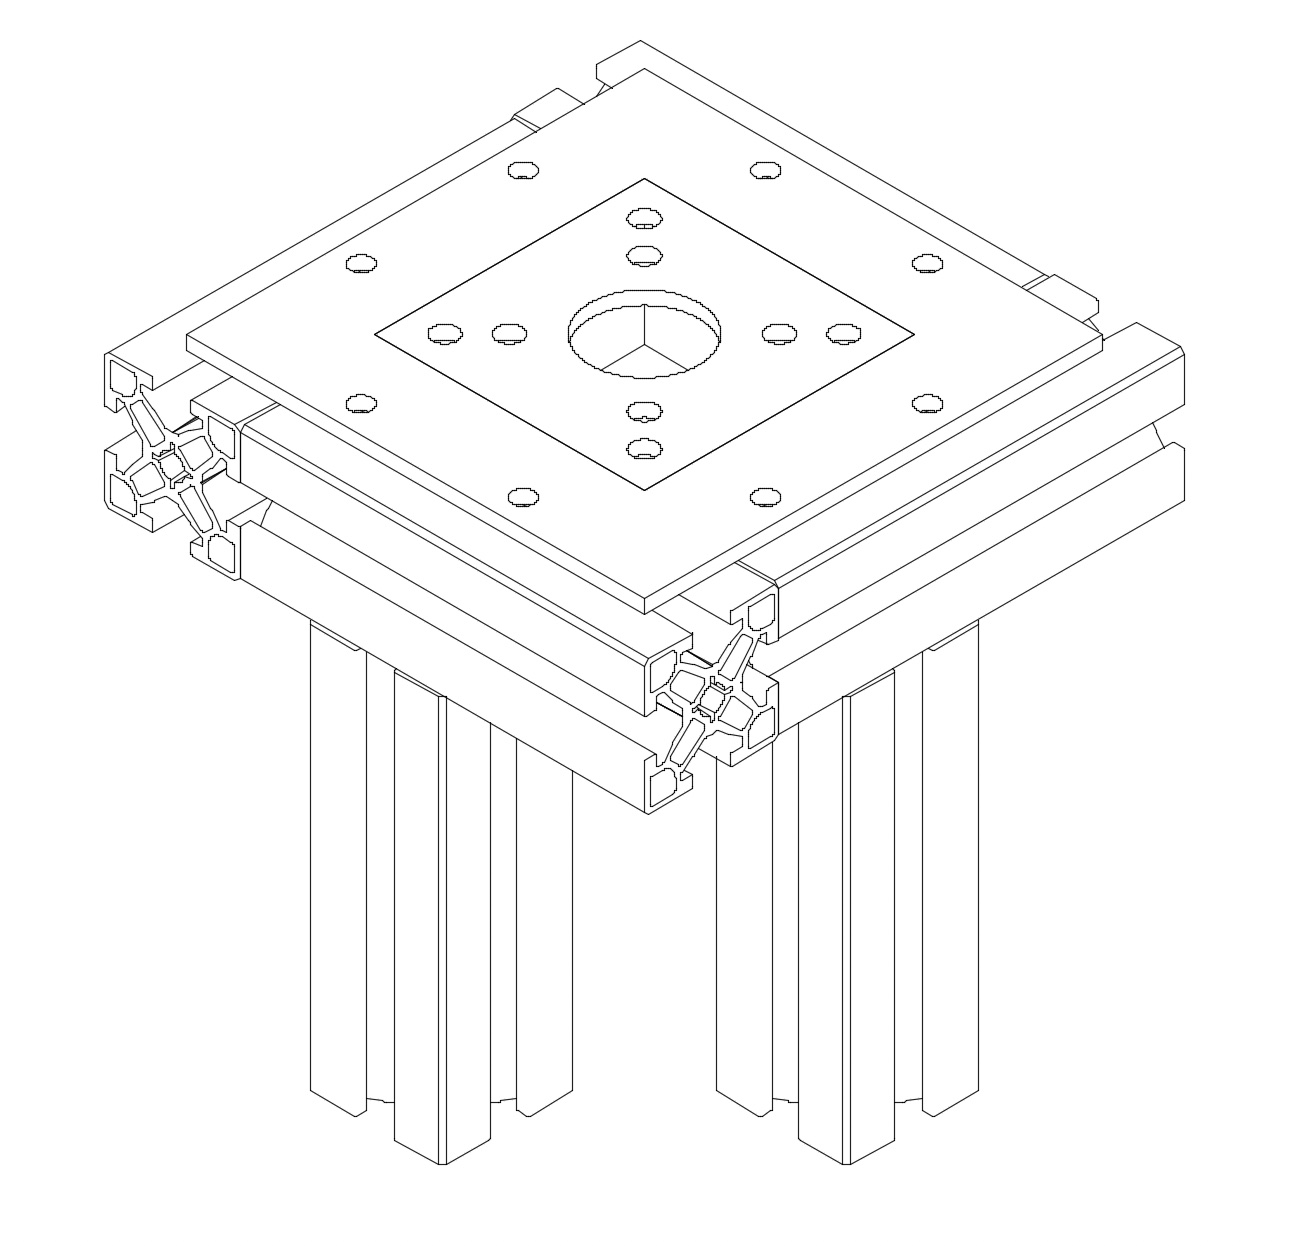
\includegraphics[height=50mm]{figures/FullThrustStand3D.jpg}
   }{%
   \vspace*{50mm}
   }
 \caption{\textit{Isometric view of the Thrust Stand Adapter with the standardised Lower Mounting Plate, as provided by the Organizer. The competitor's Upper Mounting Plate, responsible for attaching their drone to the adapter, is not depicted in the photo. Note that the design and dimensions of the Thrust Stand Plate are subject to change, but the interface for attachment, the Lower Mounting Plate, will remain unchanged.}}
 \end{figure}

\begin{enumerate}
  \item The XY-plane of the drone must be parallel to the bottom surface of the Upper Mounting Plate. Additionally, the bottom of the Upper Mounting Plate may not be positioned closer than 250mm to the drone's centre of gravity in the Z-direction.  
  \item The upper mounting plate must have four through-holes with a diameter of 9mm. They must be arranged in a two by two pattern. The teams have the opportunity to choose between two different sets of through holes:
    \begin{itemize}
      \item Smaller Set A: Four 9mm holes with a distance of ${\Delta}x=50mm$ and ${\Delta}y=50mm$.
      \item Bigger Set B: Four 9mm holes with a distance of ${\Delta}x=74mm$ and ${\Delta}y=74mm$.
    \end{itemize}
  \item The competitor's flange can not exceed the volume above the mounting plate within 200mm above the bottom of the upper mounting plate. 
  \item The design of the Upper Mounting Plate must include sufficient clearance on the top surface to allow for the placement of M8 Screws and M8 washers, per ISO 7089 standards, through the holes. The Student AirRace organisers will ensure these screws can be securely fastened on the opposite side using locknuts.
  \item The upper mounting plate and other structural mounts which only facilitate the attachment of this holding plate to the test stand may be removed by the teams for the flights. 
  \item The drone must be designed and built to transfer its thrust through the Upper Mounting Plate and its associated screws. Within the safety report, the teams must provide calculations demonstrating that their adapter can transfer the expected loads with a minimum safety factor of 5. \end{enumerate}

\begin{figure}
  \centering
  \IfFileExists{figures/ThrustStandTeamAdapterTechnicalDrawing.jpg}{%
  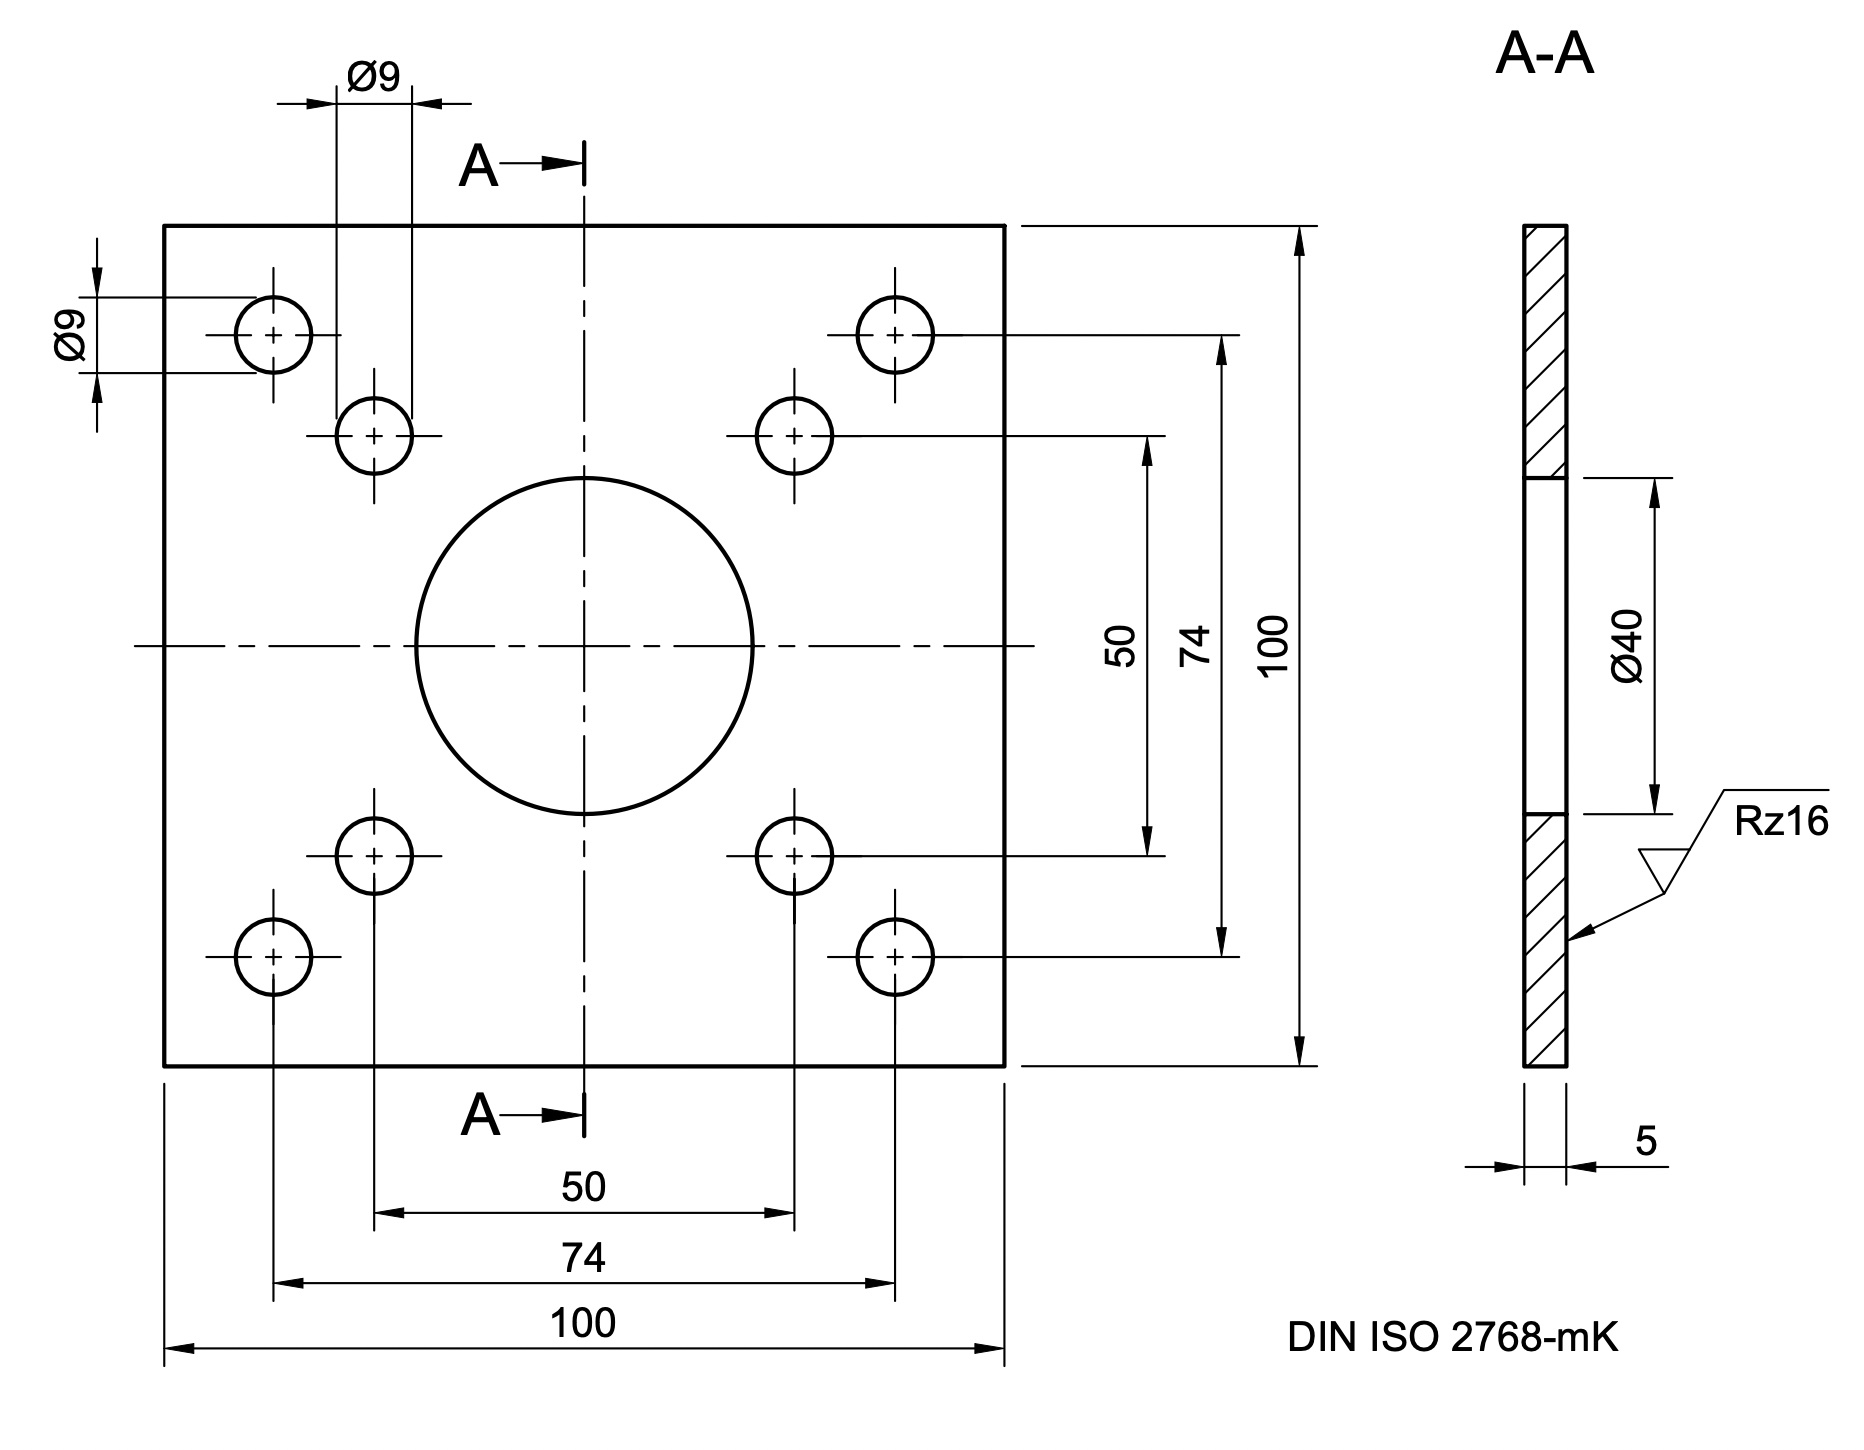
\includegraphics[height=90mm]{figures/ThrustStandTeamAdapterTechnicalDrawing.jpg}
  }{%
  \vspace*{90mm}
  }
\caption{\textit{Technical Drawing of the Lower Mounting Plate provided by the Organizer. Attention: The Adapter shown here is only the inner part of the full plate, which will be at the competition. The sidelengths will be bigger than 100mm. You cannot exceed the side lengths of 100mm.}}
\end{figure}

\begin{figure}[h!]
 \centering
  \IfFileExists{figures/ThrustStandTeamAdapter3D.jpg}{%
  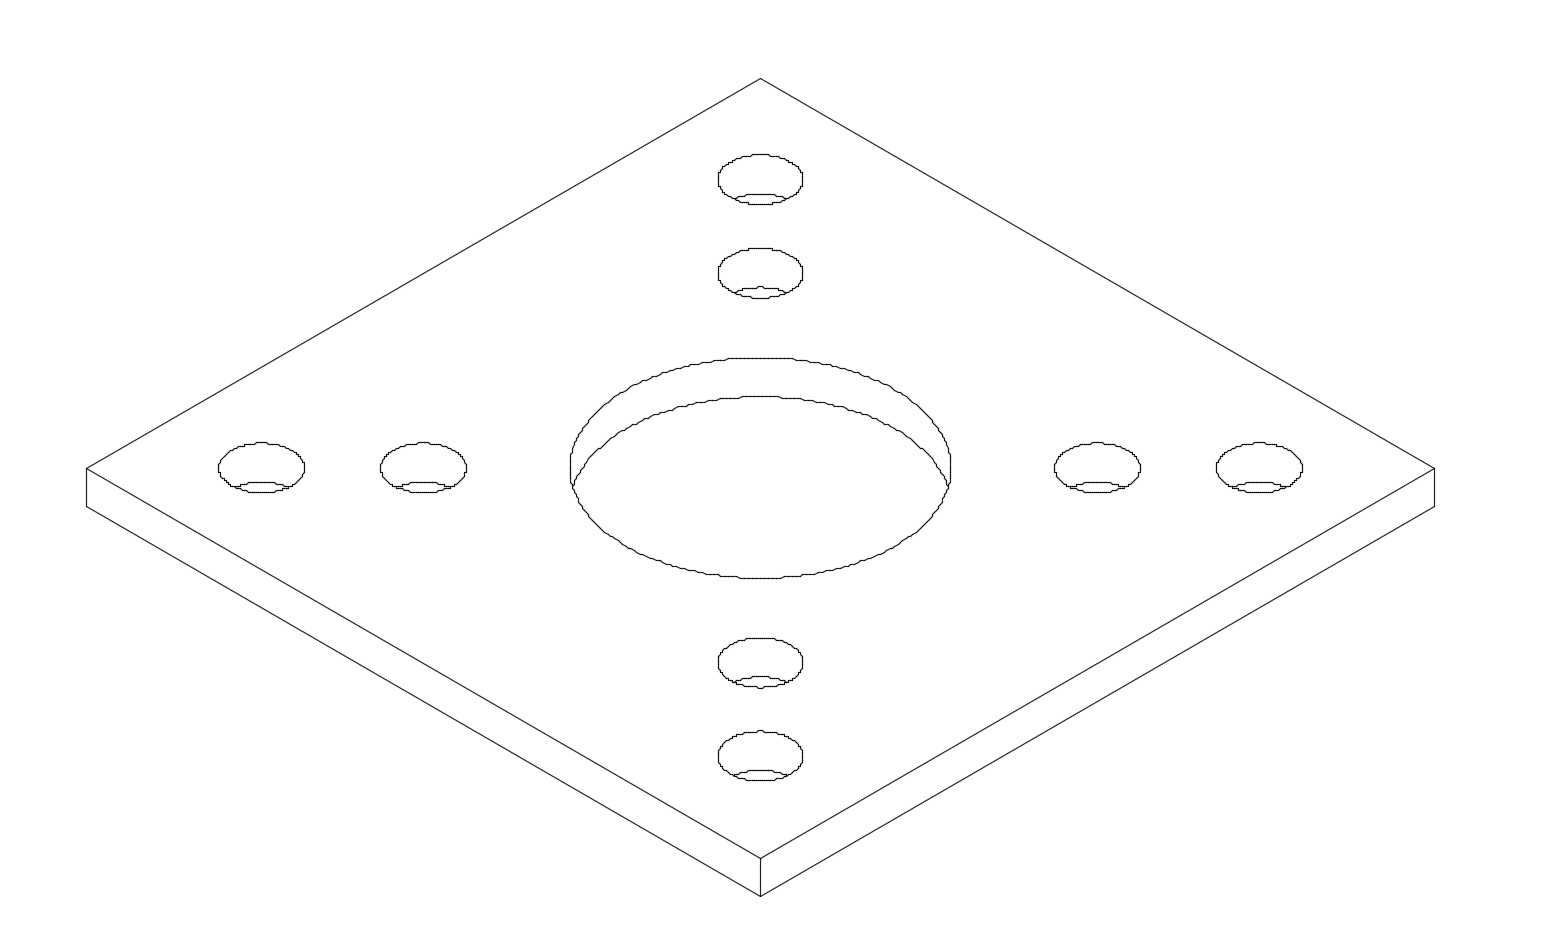
\includegraphics[height=50mm]{figures/ThrustStandTeamAdapter3D.jpg}
  }{%
  \vspace*{50mm}
  }
\caption{\textit{Isometric view of the Thruststand-Adapter.}}
\end{figure}



\subsection{Timing Equipement}
The Organizer will be responsible for measuring the race time using external optical systems such as cameras. Teams will not be required to install timing sensors or equipment within their drone. The Organizer will provide and operate the necessary timing equipment.


\section{Safety Systems}

\subsection{Shunt Plug}
The Shunt Plug is a manual and physical means for disarming the aircraft. It is supposed to completely disconnect the battery power from the motors and be able to be removed by hand in case of an emergency. We thank the Vertical Flight Society's Design-Build-Vertical Flight Competition (DBVF) for the design and inspiration behind this critical safety part. 
\begin{enumerate}
  \item A Shunt Plug must be wired between the leads of the battery system and the electronic speed controllers (or Power Distribution Device) for manual disarming and arming of the aircraft's power system.
  \item The Shunt Plug must be removable with one hand and without any tool.
  \item Installing a physical switch mounted on the drone is not permitted and will not be considered a valid Shunt Plug.
  \end{enumerate}

  \begin{figure}[h!]
    \centering
     \IfFileExists{figures/ShuntPlugA.png}{%
     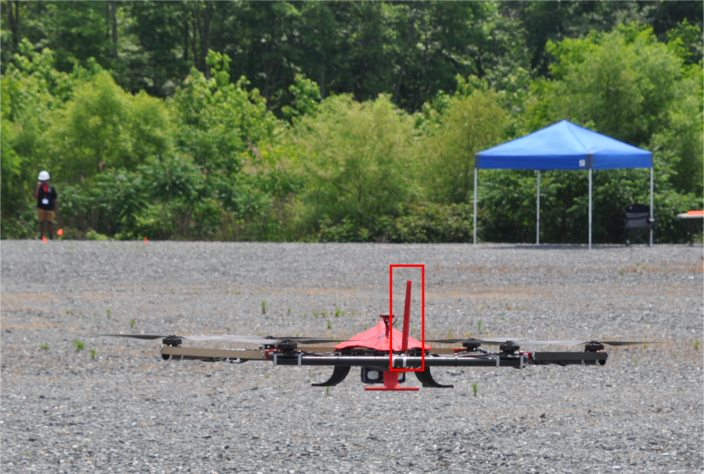
\includegraphics[height=50mm]{figures/ShuntPlugA.png}
     }{%
     \vspace*{50mm}
     }
   \caption{\textit{Shunt Plug Example (in red box) of the Buckeye Vertical Team of Ohio State University. Photo by courtesy of the Vertical Flight Society's Design-Build-Vertical Flight Competition.}}
   \end{figure}


\begin{figure}[h!]
  \centering
   \IfFileExists{figures/ShuntPlugB.png}{%
   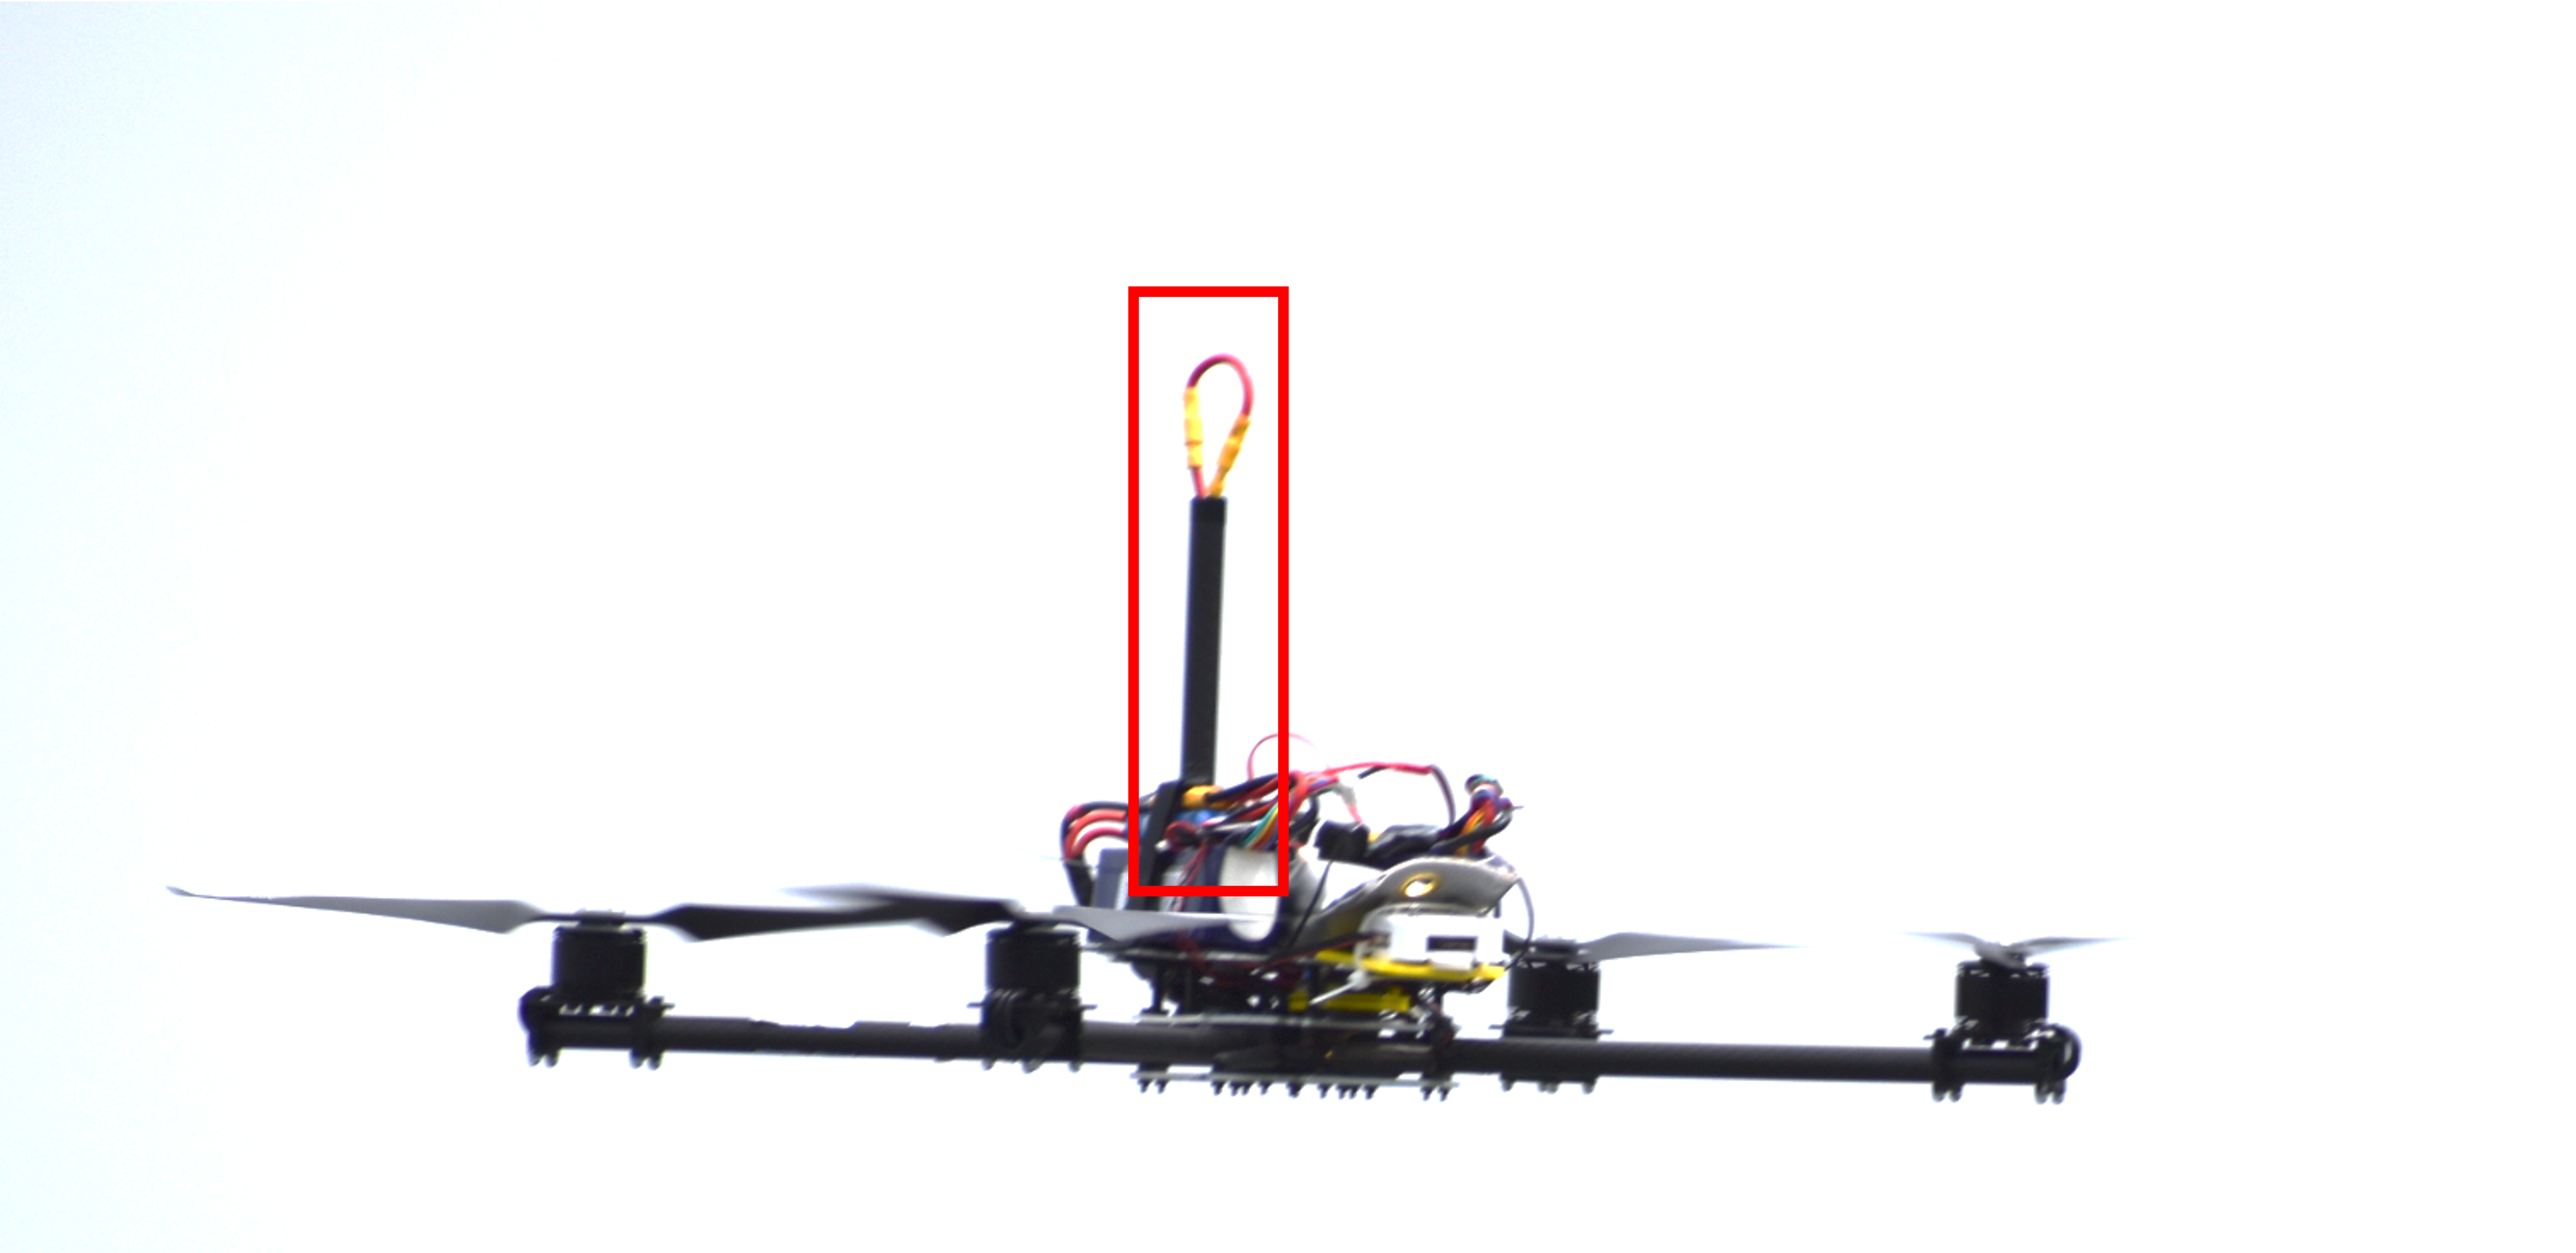
\includegraphics[height=50mm]{figures/ShuntPlugB.png}
   }{%
   \vspace*{50mm}
   }
 \caption{\textit{Shunt Plug Example (in red box) of the Autonomous Robotics Competition Club of Pennsylvania State University. Photo by courtesy of the Vertical Flight Society's Design-Build-Vertical Flight Competition.}}
 \end{figure}

  
  
  

\subsection{Ground Control Emergency Switches}
\begin{enumerate}
  \item Teams are required to have a dedicated "shutdown" switch (also commonly referred to as "kill switch") programmed into their transmitter or control console, which, when activated, must immediately shut down all flight controller motor outputs. This safety feature is mandatory for all teams participating in the competition. \\ \emph{Note: The killswitch also has to be activated in additionally to the arm switch when disconnecting the batteries manually from the UAS.}
  \item An arm/disarm switch is insufficient for a kill switch. However, the kill switch can be activated by combining multiple switches.
  \item The aircraft must be equipped with an autonomous "landing" function that allows the drone to land at its current position. A switch must be bound on the transmitter or ground station used by the team to control the aircraft that activates this landing function.  
  \item The aircraft must be equipped with an autonomous "Return to Home" (RTH) function that allows the drone to navigate back to its takeoff position. A switch must be bound on the transmitter or ground station used by the team to control the aircraft that activates this RTH function. It is important to note that the RTH process should be programmed to return the drone to a pre-determined safe location, not just the takeoff point.
  \item In addition to the dedicated switches on the transmitter or ground station, a separate and independent method of activating the emergency shutdown, autonomous landing and Return to Home (RTH) modes must be in place as a secondary means of activation. This could be achieved through alternative transmission signals, such as a standard 433MHz ground-station radio or an LTE onboard computer,  to ensure that the emergency modes can be activated even in case of failure or loss of the primary control signal.
\end{enumerate}

\subsection{Automatic Emergency Modes}
\begin{enumerate}
  \item If the transmission link between the drone and the ground station is lost, the UAV must be programmed to initiate a Return to Home automatically (RTH) emergency mode to ensure the safe return of the drone in case of lost control.
  \item The UAV must be programmed to automatically initiate a Return to Home (RTH) emergency mode if it reaches a predefined geo-zone, announced by the Organizer at the competition. This geo-zone will be defined as a multi-sided polygon, and the coordinates will be provided to the teams to ensure the safe return of the drone in case of lost control or if the aircraft reaches an area where it is no longer authorised to fly.
  \item If the flight controller allows it, teams may implement an optional automatic shutdown switch that will activate if the UAV reaches a predefined geo-zone bigger than the RTH geo-zone. This geo-zone will be defined as a multi-sided polygon, and the coordinates will be provided to the teams. The polygon will be determined based on the area that would be impacted in case of a crash and deemed as safe as possible by the Organizer. This option is an additional safety measure to protect from flyaways from the UAV.
\end{enumerate}


\subsection{Remote Emergency System}
The Organizer reserves the right to implement a remote emergency shutdown system within the avionics black box of the aircraft. However, the development of this device will likely be completed after the first competition. Therefore, teams must equip their aircraft with multiple redundant methods of turning off their drone in an emergency or losing control.

\subsection{Stratetic Mitigations}
\begin{enumerate}
  \item The aircraft must not be able to fly for longer than \textcolor{red}{60} minutes to reduce the area at risk in case of a flyaway.
  \item To enhance safety and situational awareness, a spotter must always stand next to the pilot, especially when flying in First Person View (FPV). The spotter's role is to assist the pilot by maintaining a visual on the UAV's flight path, monitoring the airspace and providing an additional set of eyes to detect any potential hazards. 
\end{enumerate}

\section{Safety Design}
Given that the competition is already set up in a manner compliant with legal regulations for drone operations, it may not be easy to establish specific and quantitative safety regulations. However, the Organizer has still implemented specific guidelines to ensure the safety of all participants. We strongly encourage teams to make every effort to follow these guidelines as closely as possible to ensure the safety of all those involved in the competition. 
\\ \\ 
However is important to note that safety processes, such as this one, are often qualitative in nature. The Organizer will strive to ensure that the safety guidelines are applied consistently and fairly for all competitors, using the EASA SORA process as a guideline as much as possible, as it will positively impact the safety report. The Organizer will take the necessary steps to review and evaluate the safety of each drone individually. To ensure safe and fair competition for all teams,   treatment will be similar across all competitors, with the same degree of scrutiny and attention to detail.

\begin{enumerate}
  \item The design and construction of the drone must have no single points of failure that would result in a crash with a catastrophic outcome. Through design calculations, simulations, and testing, teams must demonstrate that the drone can safely operate even in a failure. Any drone deemed to have a single point of failure that would lead to a crash with a catastrophic outcome will not be permitted to compete. \\ \\
  The rule for no single cause for failure shall include specifically the following points:
    \begin{itemize}
      \item Lift provided by the motors
      \item Power systems
      \item Emergency modes
      \item Video signal
      \item Transmitter/Control  (especially Receiver)
      \item Fly Away Protection 
    \end{itemize}
  It is also worth noting that this list is incomplete, and teams should consider other possible failure points for their drone design.
  \item It is recognised that eliminating all single points of failure that could lead to a crash with a catastrophic outcome may not be feasible due to cost constraints. However, teams are expected to have implemented multiple safety systems in their drone design to minimise the risk of harm to individuals on the ground. Additionally, the Organizer will have safety measures to help mitigate risk during the event.
  \item Teams must use state-of-the-art or advanced technology to design and construct their drone.
  \item Where applicable and possible, teams are encouraged to use standards and norms in the design and construction of their drone. Adhering to standards and models, such as those established by EASA, EUROCAE or ARP documents Etc., can positively impact the safety report. Teams should reference any standards and norms used in their design in the safety report.
  \item Any attempts to circumvent or subvert the safety regulations for the competition will not be tolerated. Such efforts include but are not limited to attempting to bypass safety checks, falsifying safety reports, and using non-compliant equipment. Any team that violates these regulations will be immediately disqualified from the competition without exception and may face further consequences as deemed appropriate by the Organizer.
  \item The Organizers strongly recommend that teams adhere to the processes established within the EASA SORA (Specific Operations Risk Assessment) process outlined in the EU ordinance 2019/947. Compliance with this process can aid teams in identifying and mitigating safety risks associated with their drone operation and demonstrate to the Organizers a commitment to safety. Adherence to SORA is not mandatory, but following it will positively impact the safety report.
\end{enumerate}


\section{Regulatory Requirements}
It is important to note that all competing UAVs must comply with German drone laws during the final competition, which primarily aligns with the EU open drone regulations. The Organizer will provide a summary of these regulations to assist teams in understanding and adhering to them, but it is ultimately the responsibility of each team to ensure compliance. \\ \\
Please be aware that the information provided within this document may not be exhaustive and complete, and the Organizer does not take any responsibility for the completeness and relevancy of the information provided. Teams must research and understand all applicable laws and regulations relevant to their UAV operations in Germany.
\begin{enumerate}
  \item The aircraft and their operation must be certified within the EASA A3 class in Germany. To fall within this class, a self-built aircraft must follow the rules set out by the authorities. 
  The following points include some of them yet do not include all information necessary. Competitors will need to do their research and make sure to keep up to date with the regulatory requirement on their own:
  \item Analog video signals are only allowed on certain frequency channels between 5725MHz and 5875MHz, and must not exceed an equivalent isotropically radiated power (EIRP) of 25mW.
  \item All Remote Control (RC) transmitters must have an EU Listen before talk (EU-LBT) option and hold a CE certification. Teams must declare conformity to this certification and present it to the organisers at the competition.
  \item To ensure compliance with regulatory standards, all other radio transmitters, including radio, telemetry, and video transmitters, must hold a CE certification. Teams must be prepared to present the declaration of conformity for these certifications upon request by the organisers.
  \item The aircraft's maximum takeoff weight (MTOW) must not exceed 25kg.
  \item While pilots are required to fly the aircraft within line of sight, they may use a screen or FPV goggles as long as a secondary spotter is present to assist them.
  \item It is mandatory for all drones to have a commercial drone insurance policy with a minimum coverage of 750,000 SDZ.
  \item The aircraft must be registered with EASA or in Germany and have an e-ID.
  \item The aircraft must also have a fireproof badge displaying the EASA e-ID of the vehicle operator.
  \item To participate, pilots must hold a valid EASA A1/A3 license and be at least 16 years of age.
\end{enumerate}

\section{Additional Requirements}
To enhance safety and professionalism and align the competition with real-world aviation practices, the organisers have established additional regulations that teams must adhere to. These regulations are not specific to the A3 class but are based on other aviation standards and the SORA process. Compliance with these regulations is mandatory for all teams participating in the competition.

\begin{enumerate}
  \item It is required that flight books and documentation are completed and maintained for each flight to accurately record and track the flight hours and experiences of the pilots and aircraft.
  \item To ensure the safety and regulatory compliance of the competition, standard and emergency checklists and an emergency response plan must be in place and followed for every flight.
  \item Before takeoff, pilots must gather and review relevant Notice To Air Missions (NOTAMS), airspace information, and weather conditions to ensure the planned flight can be safely conducted.
  \item After being accepted into the competition, the teams will receive a specialised weather forecasting and analysis tool. This tool was developed specifically for professional aviation by one of the competition partners. 
  This tool will allow the teams to accurately assess and predict the weather conditions they will encounter during their test flights and development, helping to ensure the safety and success of their operations. 
  \item All off-the-shelf electronic components used in the competition must be CE certified to meet necessary safety and performance standards.
  \item The competition teams are expected to foster a "just culture" within their organisation, promoting the reporting of incidents and a focus on safety. \textcolor{red}{Student AirRace is also seeking to provide the teams with workshops about this topic.}
  \item Following each flight, the team must write a report detailing any issues or concerns that arose during the flight. It can be submitted to the Organizer to give them feedback on their rules and the team's current process.
\end{enumerate}







\end{document}